\documentclass[landscape]{infslides}
\usepackage{graphicx}
\usepackage{multicol}
\usepackage[export]{adjustbox}
\def\ps@nofooter{\let\@mkboth\markboth
\def\@oddfoot{\empty}%
\def\@oddhead{\@tempdima=\textwidth \advance\@tempdima-45mm
            \vbox{\setcolour{\bar@colour}\hrule \@depth3pt
                \@width\@tempdima \vskip1.5pt \setcolour{\info@colour}
                    \hbox to\@tempdima{\footnotesize\csslide@font
                                        \extra@info\hfill\thepage}}%
            \vbox to\z@{\vss\hbox to45mm{
                \resizebox{45mm}{!}{\includegraphics{school_of_informatics}}\hss}\vss
                \vskip2\headheight}}%
\def\@evenfoot{\@oddfoot}%
\def\@evenhead{\@oddhead}}
\graphicspath{{./images/}}
\begin{document}

\title[IoTSSC Project]{IoTSSC Project\\Indoor Localisation}
\author[Lorenzo Martinico and Piotr Jander]{Lorenzo Martinico \and Piotr Jander}
\date{\today}

\maketitle
%\tableofcontents
\begin{slide}{Tracking device}
    Our chosen localisation device is a Nordic nRF51-DK, running ARM Mbed OS 5
    \begin{figure}
        \centering
        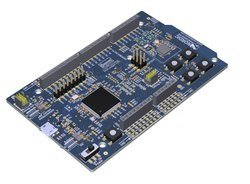
\includegraphics{nRF51-DK.jpg}
    \end{figure}
    Due to limited processing power, the firmware running on the board is limitied to scanning for Bluetooth Beacons and updating a BLE Characteristic with their RSSI strength
\end{slide}
\begin{slide}{Android App}
    \thispagestyle{nofooter}
    \begin{multicols}{2}
        The app acts as a Bluetooth gateway, connecting to the board to read from its LocationService, and forward a timestamped RSSI, BeaconID pair to the server.\\
        Additionally, we display a map of the 5th floor, and a location marker, which can be manually modified based on the board's position to collect training data.
        \begin{figure}
            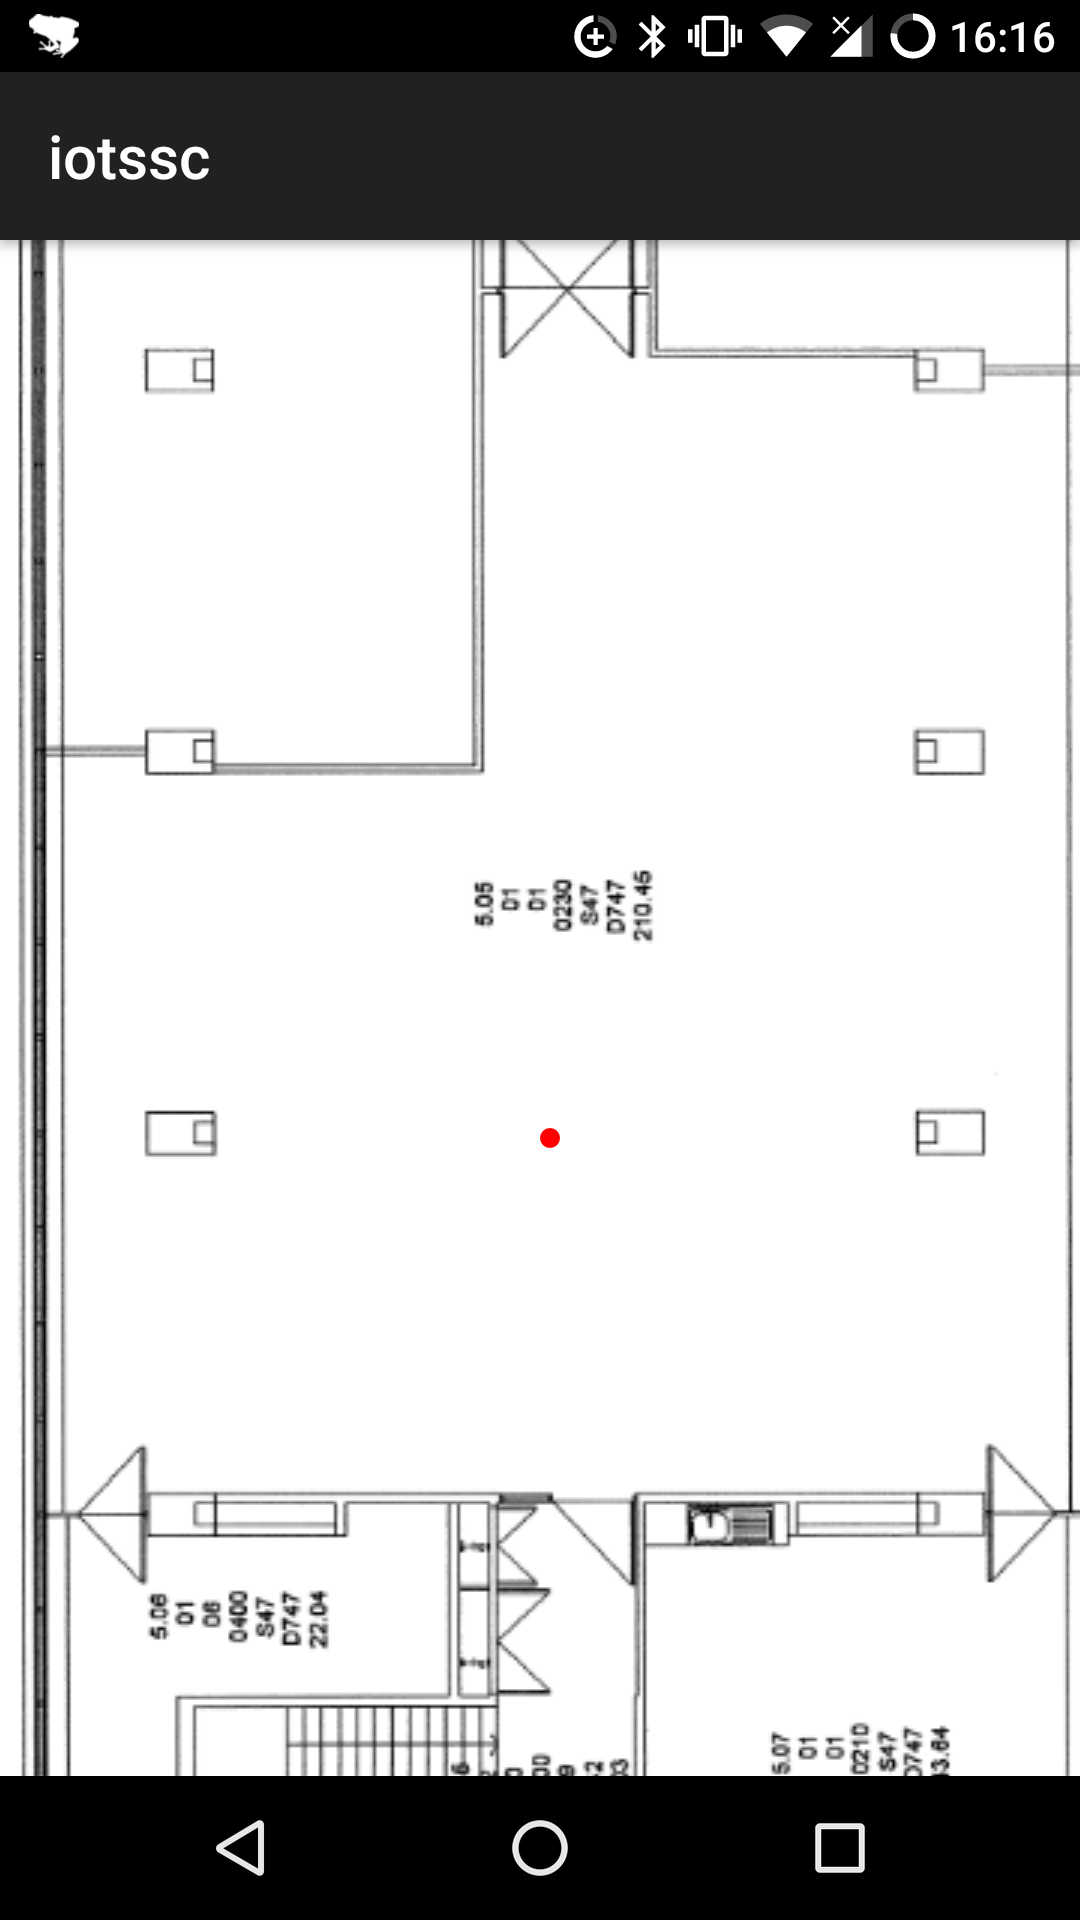
\includegraphics[scale=0.2,right]{Screenshot.png}
        \end{figure}
    \end{multicols}
\end{slide}
\begin{slide}{Server}
The server is a simple Flask app hosted on a Google Cloud Virtual Machine. It receives POST requests from the Gateway, and saves the data in a file.

To ensure all data is transimitted securely, the server runs over HTTPS, using a self signed certificate manually provisioned to the app (its only client).
\end{slide}
\begin{slide}{Analytics}
    ...
    RSSI triangulation 
    SVMs
    KNN
    Kalman Filters
\end{slide}
\begin{slide}{Collected data}
    \thispagestyle{nofooter}
    
    \begin{multicols}{2}
    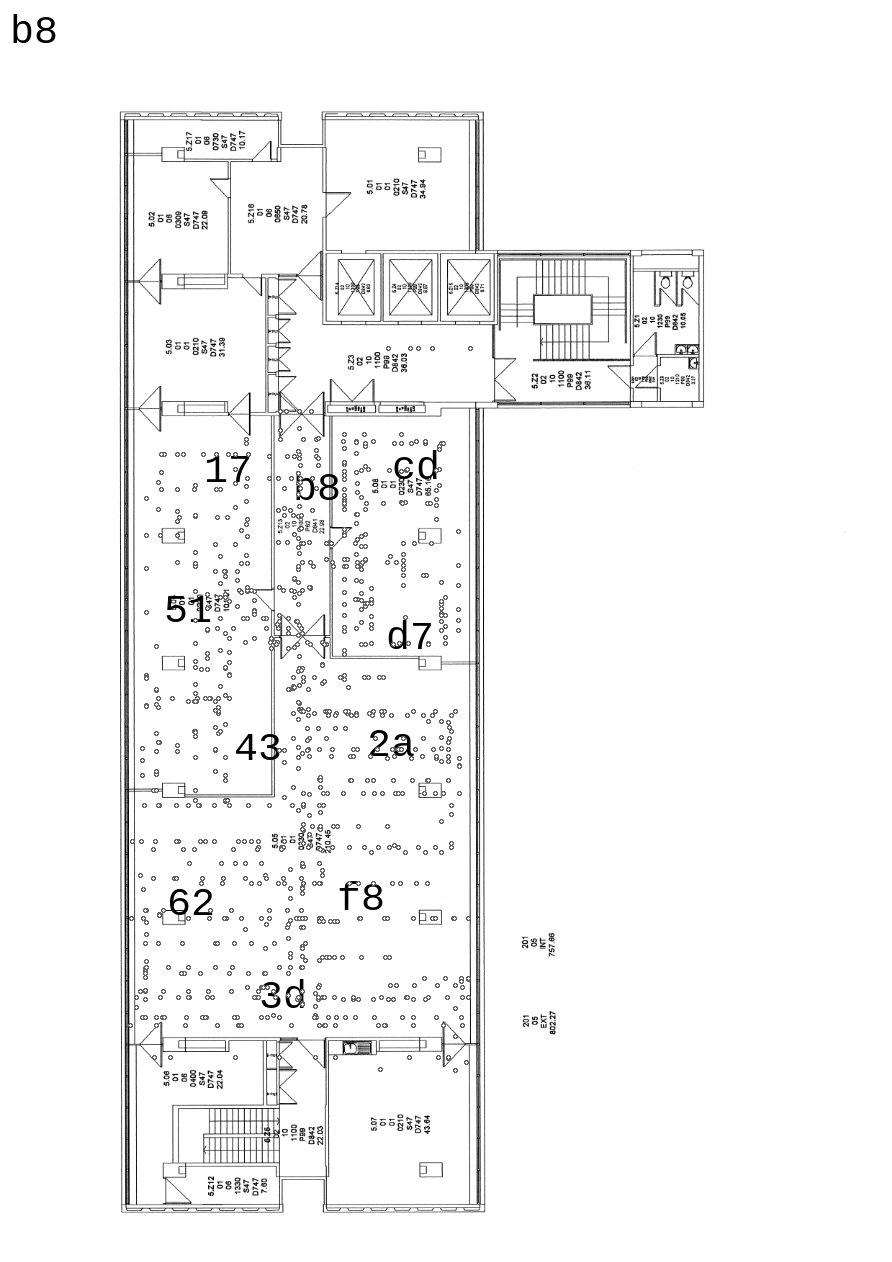
\includegraphics[width=0.9\linewidth]{b8_read.png}
    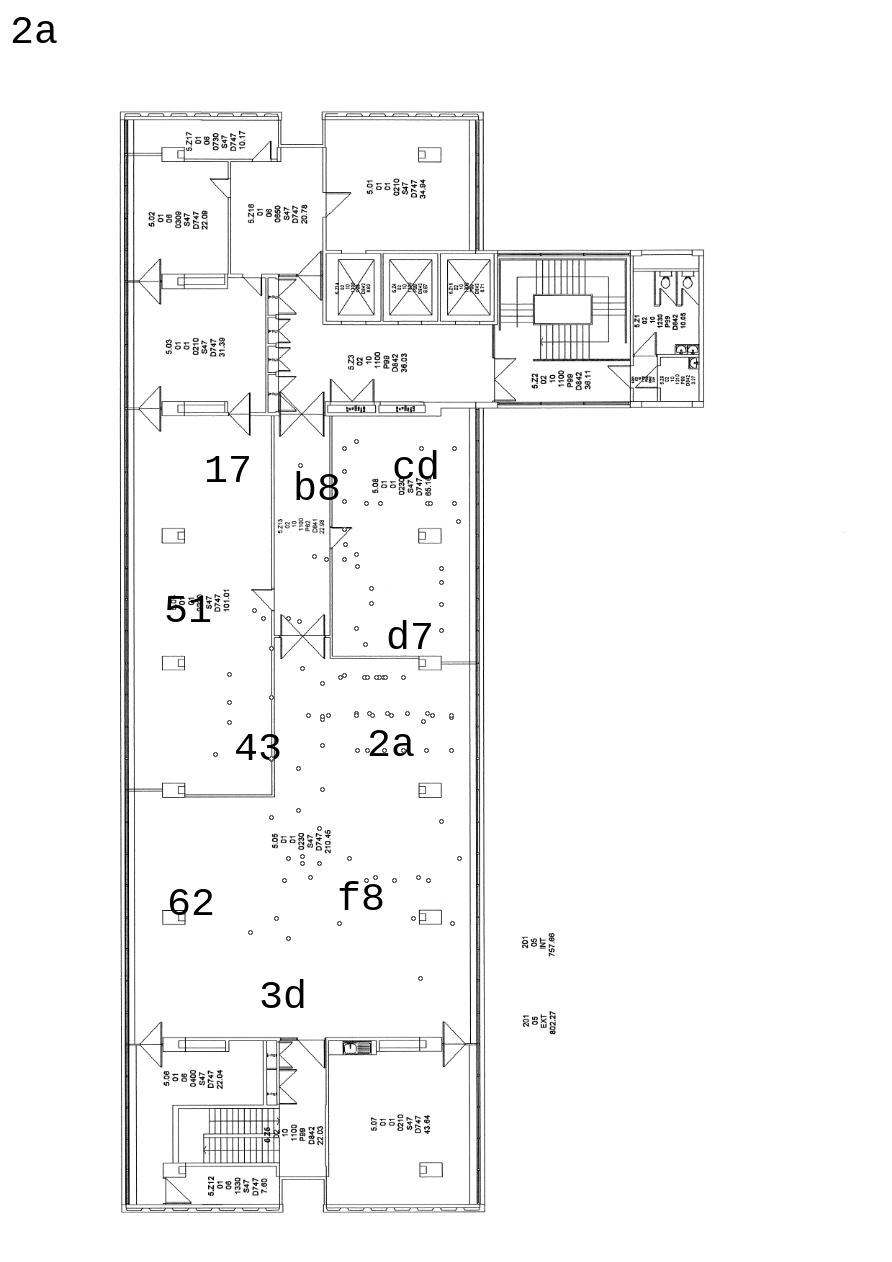
\includegraphics[width=0.9\linewidth]{2a_read.png}
    \end{multicols}
\end{slide}

\begin{slide}{Conversion to/from global coordinates}
\begin{itemize}
\item We need to convert between global coordinates and pixel coordinates.
\item For the tiny area of a building, we can approximate spherical coordinates with Cartesian coordinates.
\item We translate the coordinates vectors so that the origin is at the NE corner of the floor, and then perform rotation and scaling by multiply a vector by a 2x2 matrix (or its inverse).
\item The conversion matrix was found by taking the global / pixel coordinates of three points and solving a linear equation.
\end{itemize}
\end{slide}

\begin{slide}{Does free-space propagation model hold?}
    \thispagestyle{nofooter}
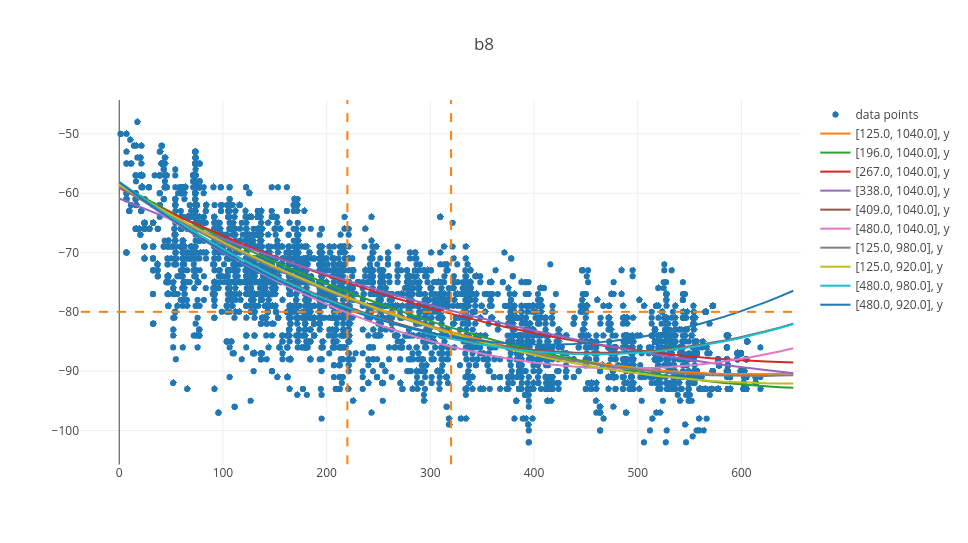
\includegraphics[height=0.84\textheight,width=\textwidth]{images/different_directions.png}
\end{slide}

\begin{slide}{Idea: trilateration on beacons 17 and b8}
    \centering
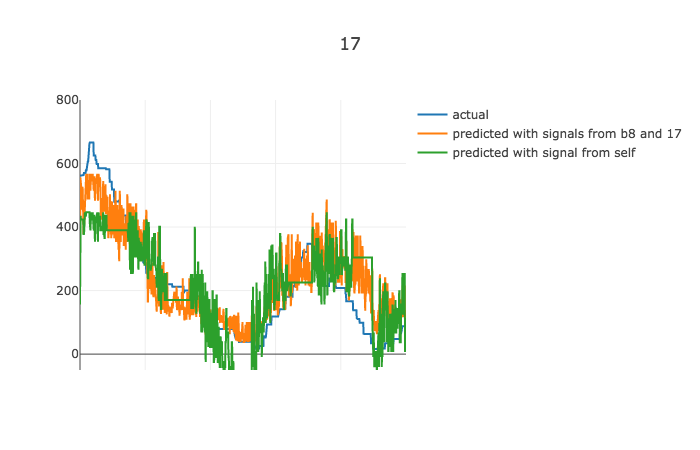
\includegraphics[width=0.55\linewidth]{images/dist_f_rssi_17.png}

We fit a quadratic polynomial to find distance from 17 and b8 as a function of signal strength. A polynomial in two variables gives slightly better results, giving an average error of 4 meters rather than 5 meters.
\end{slide}

\begin{slide}{Idea: trilateration on beacons 17 and b8}
    \centering
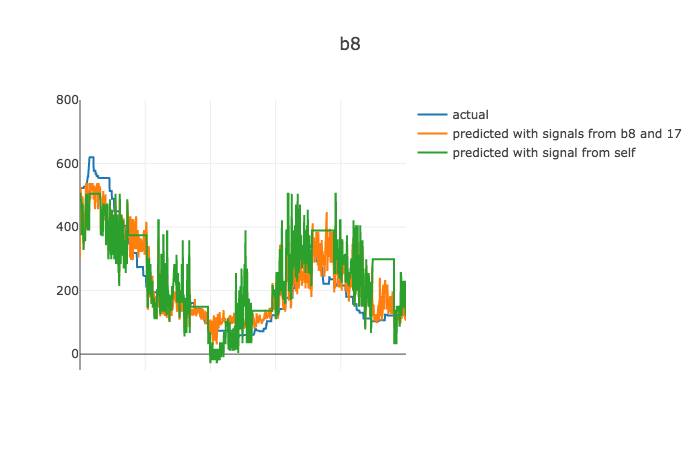
\includegraphics[width=0.55\linewidth]{images/dist_f_rssi_b8.png}

Once we have an estimate of the distance, we can perform trilateration using the law of cosines. If we were using signals from more than two beacons, trilateration would require expensive least squares regression.
\end{slide}

\begin{slide}{Localisation with triangulation}
    \centering
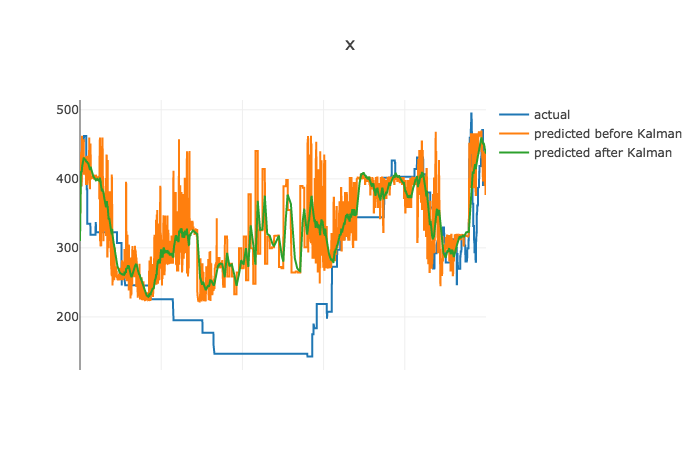
\includegraphics[width=0.6\linewidth]{images/trilateration_x.png}

A test using the triangulation method gives error of more than 4 meters.
\end{slide}

\begin{slide}{Localisation with triangulation}
    \centering
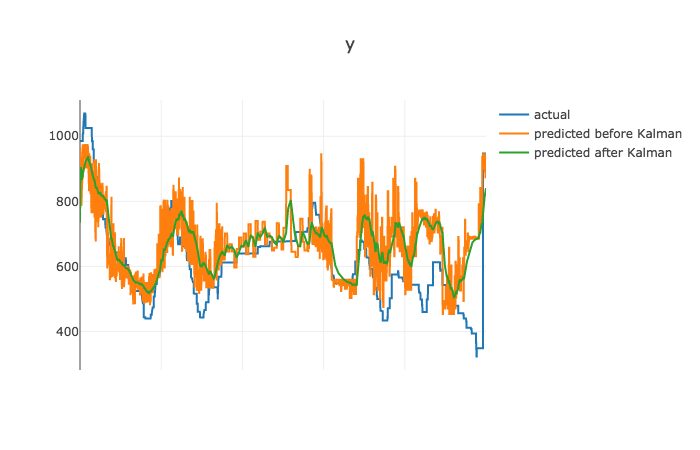
\includegraphics[width=0.6\linewidth]{images/trilateration_y.png}

Accuracy could be improved by incorporating signal strength from other beacons.
\end{slide}

\begin{slide}{Localisation with triangulation}
    \centering{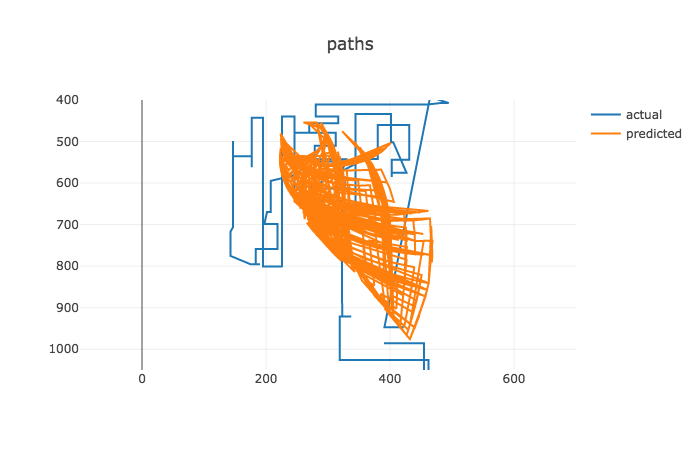
\includegraphics[width=0.6\linewidth]{images/trilateration_path_no_kalman.png}}

Foobar
\end{slide}

\begin{slide}{Localisation with triangulation}
    \centering
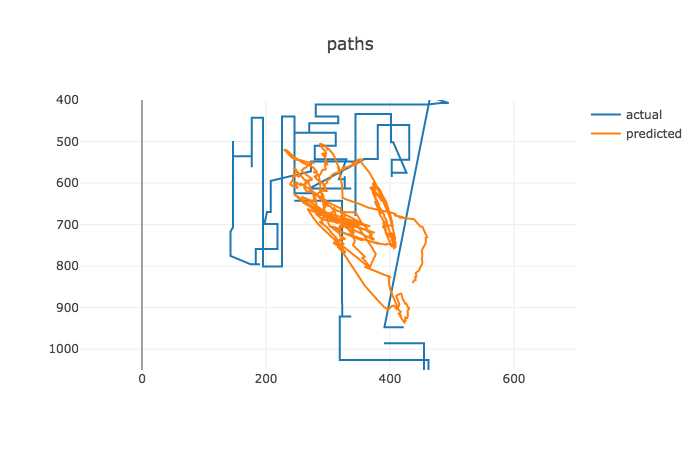
\includegraphics[width=0.6\linewidth]{images/trilateration_path.png}

Applying a Kalman filter only gives slight improvements in numerical terms, but the path looks more plausible.
\end{slide}

\end{document}












